\documentclass[1p]{elsarticle_modified}
%\bibliographystyle{elsarticle-num}

%\usepackage[colorlinks]{hyperref}
%\usepackage{abbrmath_seonhwa} %\Abb, \Ascr, \Acal ,\Abf, \Afrak
\usepackage{amsfonts}
\usepackage{amssymb}
\usepackage{amsmath}
\usepackage{amsthm}
\usepackage{scalefnt}
\usepackage{amsbsy}
\usepackage{kotex}
\usepackage{caption}
\usepackage{subfig}
\usepackage{color}
\usepackage{graphicx}
\usepackage{xcolor} %% white, black, red, green, blue, cyan, magenta, yellow
\usepackage{float}
\usepackage{setspace}
\usepackage{hyperref}

\usepackage{tikz}
\usetikzlibrary{arrows}

\usepackage{multirow}
\usepackage{array} % fixed length table
\usepackage{hhline}

%%%%%%%%%%%%%%%%%%%%%
\makeatletter
\renewcommand*\env@matrix[1][\arraystretch]{%
	\edef\arraystretch{#1}%
	\hskip -\arraycolsep
	\let\@ifnextchar\new@ifnextchar
	\array{*\c@MaxMatrixCols c}}
\makeatother %https://tex.stackexchange.com/questions/14071/how-can-i-increase-the-line-spacing-in-a-matrix
%%%%%%%%%%%%%%%

\usepackage[normalem]{ulem}

\newcommand{\msout}[1]{\ifmmode\text{\sout{\ensuremath{#1}}}\else\sout{#1}\fi}
%SOURCE: \msout is \stkout macro in https://tex.stackexchange.com/questions/20609/strikeout-in-math-mode

\newcommand{\cancel}[1]{
	\ifmmode
	{\color{red}\msout{#1}}
	\else
	{\color{red}\sout{#1}}
	\fi
}

\newcommand{\add}[1]{
	{\color{blue}\uwave{#1}}
}

\newcommand{\replace}[2]{
	\ifmmode
	{\color{red}\msout{#1}}{\color{blue}\uwave{#2}}
	\else
	{\color{red}\sout{#1}}{\color{blue}\uwave{#2}}
	\fi
}

\newcommand{\Sol}{\mathcal{S}} %segment
\newcommand{\D}{D} %diagram
\newcommand{\A}{\mathcal{A}} %arc


%%%%%%%%%%%%%%%%%%%%%%%%%%%%%5 test

\def\sl{\operatorname{\textup{SL}}(2,\Cbb)}
\def\psl{\operatorname{\textup{PSL}}(2,\Cbb)}
\def\quan{\mkern 1mu \triangleright \mkern 1mu}

\theoremstyle{definition}
\newtheorem{thm}{Theorem}[section]
\newtheorem{prop}[thm]{Proposition}
\newtheorem{lem}[thm]{Lemma}
\newtheorem{ques}[thm]{Question}
\newtheorem{cor}[thm]{Corollary}
\newtheorem{defn}[thm]{Definition}
\newtheorem{exam}[thm]{Example}
\newtheorem{rmk}[thm]{Remark}
\newtheorem{alg}[thm]{Algorithm}

\newcommand{\I}{\sqrt{-1}}
\begin{document}

%\begin{frontmatter}
%
%\title{Boundary parabolic representations of knots up to 8 crossings}
%
%%% Group authors per affiliation:
%\author{Yunhi Cho} 
%\address{Department of Mathematics, University of Seoul, Seoul, Korea}
%\ead{yhcho@uos.ac.kr}
%
%
%\author{Seonhwa Kim} %\fnref{s_kim}}
%\address{Center for Geometry and Physics, Institute for Basic Science, Pohang, 37673, Korea}
%\ead{ryeona17@ibs.re.kr}
%
%\author{Hyuk Kim}
%\address{Department of Mathematical Sciences, Seoul National University, Seoul 08826, Korea}
%\ead{hyukkim@snu.ac.kr}
%
%\author{Seokbeom Yoon}
%\address{Department of Mathematical Sciences, Seoul National University, Seoul, 08826,  Korea}
%\ead{sbyoon15@snu.ac.kr}
%
%\begin{abstract}
%We find all boundary parabolic representation of knots up to 8 crossings.
%
%\end{abstract}
%\begin{keyword}
%    \MSC[2010] 57M25 
%\end{keyword}
%
%\end{frontmatter}

%\linenumbers
%\tableofcontents
%
\newcommand\colored[1]{\textcolor{white}{\rule[-0.35ex]{0.8em}{1.4ex}}\kern-0.8em\color{red} #1}%
%\newcommand\colored[1]{\textcolor{white}{ #1}\kern-2.17ex	\textcolor{white}{ #1}\kern-1.81ex	\textcolor{white}{ #1}\kern-2.15ex\color{red}#1	}

{\Large $\underline{12a_{0429}~(K12a_{0429})}$}

\setlength{\tabcolsep}{10pt}
\renewcommand{\arraystretch}{1.6}
\vspace{1cm}\begin{tabular}{m{100pt}>{\centering\arraybackslash}m{274pt}}
\multirow{5}{120pt}{
	\centering
	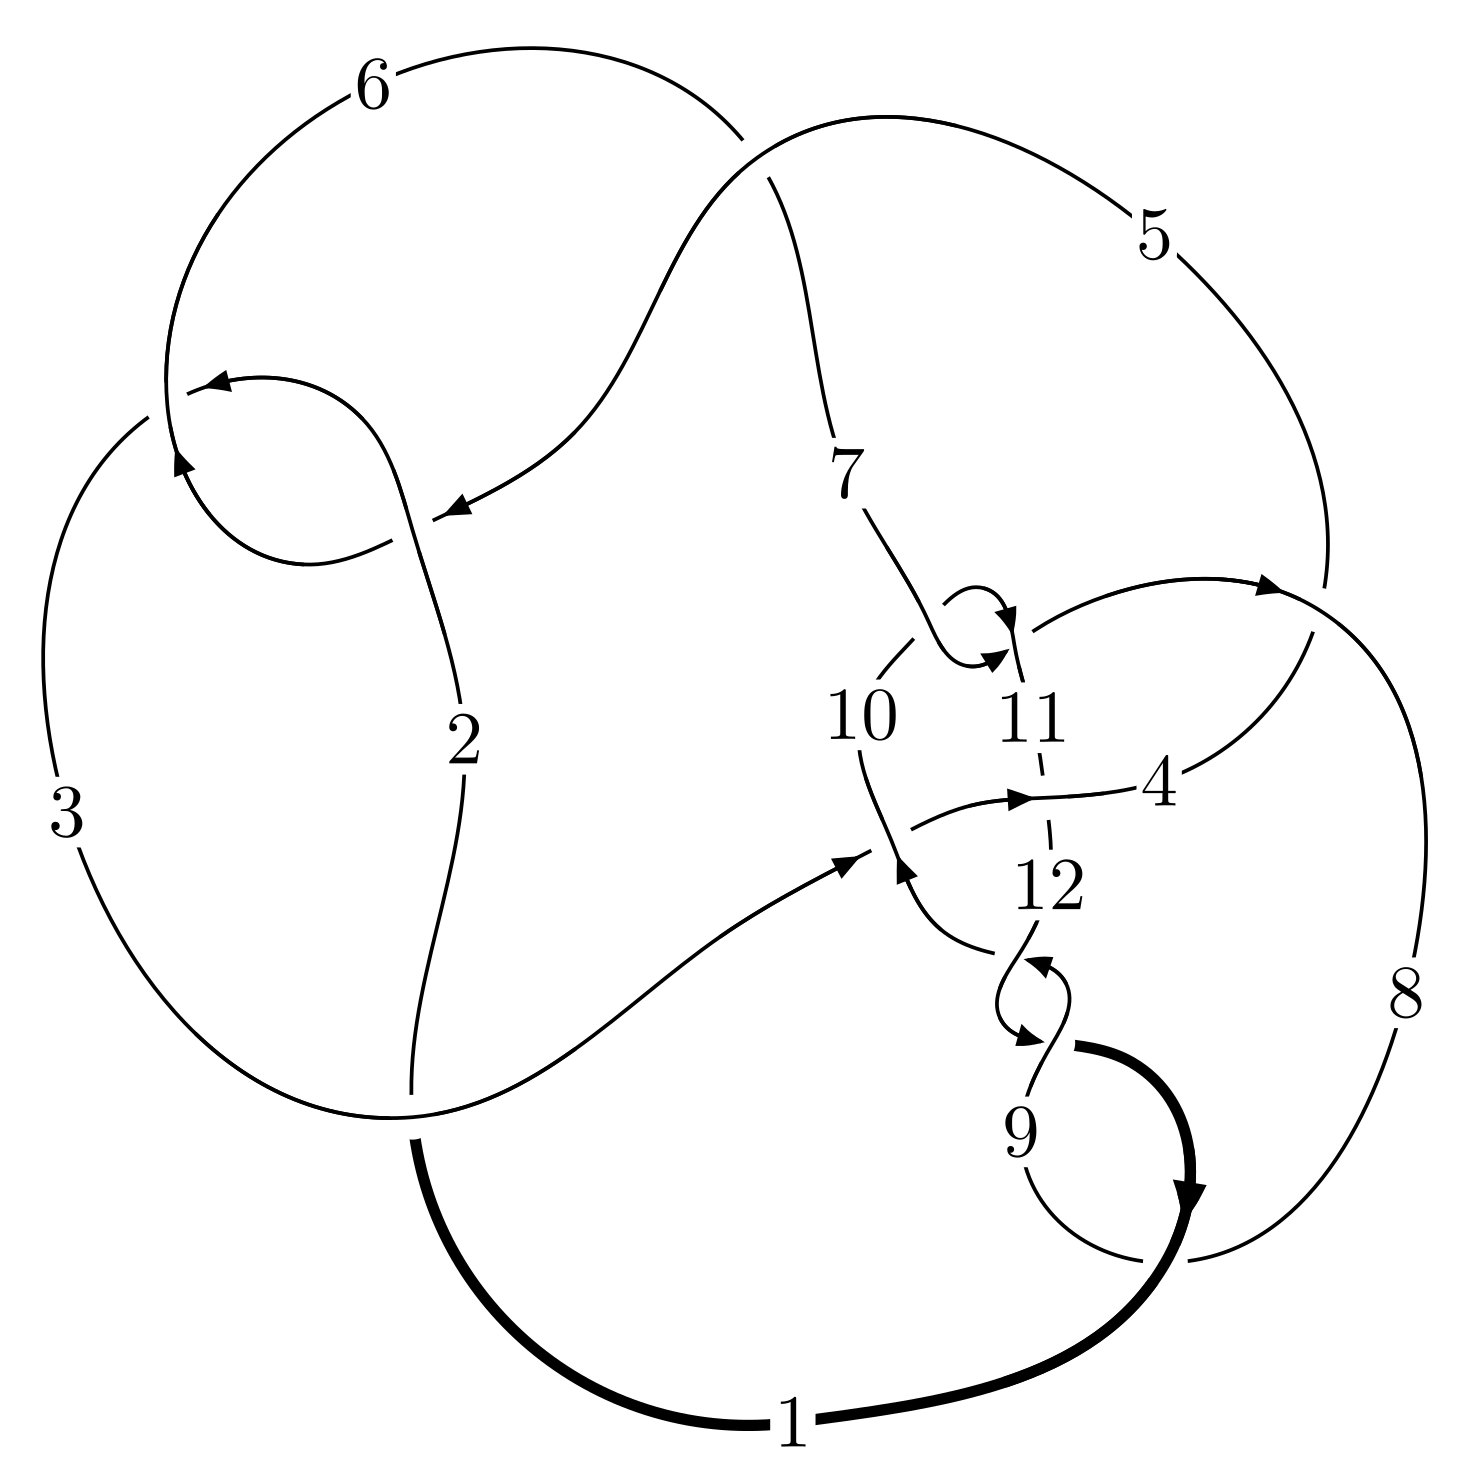
\includegraphics[width=112pt]{../../../GIT/diagram.site/Diagrams/png/1230_12a_0429.png}\\
\ \ \ A knot diagram\footnotemark}&
\allowdisplaybreaks
\textbf{Linearized knot diagam} \\
\cline{2-2}
 &
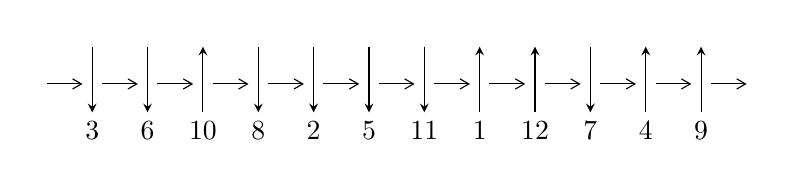
\begin{tikzpicture}[x=20pt, y=17pt]
	% nodes
	\node (C0) at (0, 0) {};
	\node (C1) at (1, 0) {};
	\node (C1U) at (1, +1) {};
	\node (C1D) at (1, -1) {3};

	\node (C2) at (2, 0) {};
	\node (C2U) at (2, +1) {};
	\node (C2D) at (2, -1) {6};

	\node (C3) at (3, 0) {};
	\node (C3U) at (3, +1) {};
	\node (C3D) at (3, -1) {10};

	\node (C4) at (4, 0) {};
	\node (C4U) at (4, +1) {};
	\node (C4D) at (4, -1) {8};

	\node (C5) at (5, 0) {};
	\node (C5U) at (5, +1) {};
	\node (C5D) at (5, -1) {2};

	\node (C6) at (6, 0) {};
	\node (C6U) at (6, +1) {};
	\node (C6D) at (6, -1) {5};

	\node (C7) at (7, 0) {};
	\node (C7U) at (7, +1) {};
	\node (C7D) at (7, -1) {11};

	\node (C8) at (8, 0) {};
	\node (C8U) at (8, +1) {};
	\node (C8D) at (8, -1) {1};

	\node (C9) at (9, 0) {};
	\node (C9U) at (9, +1) {};
	\node (C9D) at (9, -1) {12};

	\node (C10) at (10, 0) {};
	\node (C10U) at (10, +1) {};
	\node (C10D) at (10, -1) {7};

	\node (C11) at (11, 0) {};
	\node (C11U) at (11, +1) {};
	\node (C11D) at (11, -1) {4};

	\node (C12) at (12, 0) {};
	\node (C12U) at (12, +1) {};
	\node (C12D) at (12, -1) {9};
	\node (C13) at (13, 0) {};

	% arrows
	\draw[->,>={angle 60}]
	(C0) edge (C1) (C1) edge (C2) (C2) edge (C3) (C3) edge (C4) (C4) edge (C5) (C5) edge (C6) (C6) edge (C7) (C7) edge (C8) (C8) edge (C9) (C9) edge (C10) (C10) edge (C11) (C11) edge (C12) (C12) edge (C13) ;	\draw[->,>=stealth]
	(C1U) edge (C1D) (C2U) edge (C2D) (C3D) edge (C3U) (C4U) edge (C4D) (C5U) edge (C5D) (C6U) edge (C6D) (C7U) edge (C7D) (C8D) edge (C8U) (C9D) edge (C9U) (C10U) edge (C10D) (C11D) edge (C11U) (C12D) edge (C12U) ;
	\end{tikzpicture} \\
\hhline{~~} \\& 
\textbf{Solving Sequence} \\ \cline{2-2} 
 &
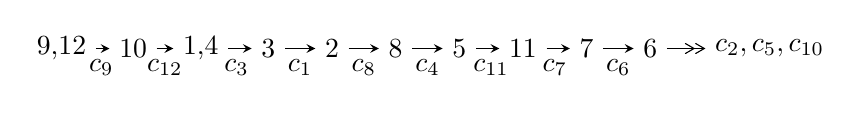
\begin{tikzpicture}[x=23pt, y=7pt]
	% node
	\node (A0) at (-1/8, 0) {9,12};
	\node (A1) at (1, 0) {10};
	\node (A2) at (33/16, 0) {1,4};
	\node (A3) at (25/8, 0) {3};
	\node (A4) at (33/8, 0) {2};
	\node (A5) at (41/8, 0) {8};
	\node (A6) at (49/8, 0) {5};
	\node (A7) at (57/8, 0) {11};
	\node (A8) at (65/8, 0) {7};
	\node (A9) at (73/8, 0) {6};
	\node (C1) at (1/2, -1) {$c_{9}$};
	\node (C2) at (3/2, -1) {$c_{12}$};
	\node (C3) at (21/8, -1) {$c_{3}$};
	\node (C4) at (29/8, -1) {$c_{1}$};
	\node (C5) at (37/8, -1) {$c_{8}$};
	\node (C6) at (45/8, -1) {$c_{4}$};
	\node (C7) at (53/8, -1) {$c_{11}$};
	\node (C8) at (61/8, -1) {$c_{7}$};
	\node (C9) at (69/8, -1) {$c_{6}$};
	\node (A10) at (11, 0) {$c_{2},c_{5},c_{10}$};

	% edge
	\draw[->,>=stealth]	
	(A0) edge (A1) (A1) edge (A2) (A2) edge (A3) (A3) edge (A4) (A4) edge (A5) (A5) edge (A6) (A6) edge (A7) (A7) edge (A8) (A8) edge (A9) ;
	\draw[->>,>={angle 60}]	
	(A9) edge (A10);
\end{tikzpicture} \\ 

\end{tabular} \\

\footnotetext{
The image of knot diagram is generated by the software ``\textbf{Draw programme}" developed by Andrew Bartholomew(\url{http://www.layer8.co.uk/maths/draw/index.htm\#Running-draw}), where we modified some parts for our purpose(\url{https://github.com/CATsTAILs/LinksPainter}).
}\phantom \\ \newline 
\centering \textbf{Ideals for irreducible components\footnotemark of $X_{\text{par}}$} 
 
\begin{align*}
I^u_{1}&=\langle 
-2.05234\times10^{155} u^{99}+7.99874\times10^{155} u^{98}+\cdots+1.26559\times10^{156} b-4.31298\times10^{155},\\
\phantom{I^u_{1}}&\phantom{= \langle  }-6.46036\times10^{154} u^{99}+2.42368\times10^{155} u^{98}+\cdots+4.21862\times10^{155} a-2.87887\times10^{155},\\
\phantom{I^u_{1}}&\phantom{= \langle  }u^{100}-4 u^{99}+\cdots-2 u+2\rangle \\
I^u_{2}&=\langle 
9 b^3+6 b^2 u+3 b^2-6 b-2 u-1,\;a,\;u^2+u+1\rangle \\
I^u_{3}&=\langle 
b+1,\;2 a+u,\;u^2+2\rangle \\
\\
I^v_{1}&=\langle 
a,\;b-1,\;v-1\rangle \\
\end{align*}
\raggedright * 4 irreducible components of $\dim_{\mathbb{C}}=0$, with total 109 representations.\\
\footnotetext{All coefficients of polynomials are rational numbers. But the coefficients are sometimes approximated in decimal forms when there is not enough margin.}
\newpage
\renewcommand{\arraystretch}{1}
\centering \section*{I. $I^u_{1}= \langle -2.05\times10^{155} u^{99}+8.00\times10^{155} u^{98}+\cdots+1.27\times10^{156} b-4.31\times10^{155},\;-6.46\times10^{154} u^{99}+2.42\times10^{155} u^{98}+\cdots+4.22\times10^{155} a-2.88\times10^{155},\;u^{100}-4 u^{99}+\cdots-2 u+2 \rangle$}
\flushleft \textbf{(i) Arc colorings}\\
\begin{tabular}{m{7pt} m{180pt} m{7pt} m{180pt} }
\flushright $a_{9}=$&$\begin{pmatrix}1\\0\end{pmatrix}$ \\
\flushright $a_{12}=$&$\begin{pmatrix}0\\u\end{pmatrix}$ \\
\flushright $a_{10}=$&$\begin{pmatrix}1\\- u^2\end{pmatrix}$ \\
\flushright $a_{1}=$&$\begin{pmatrix}u\\u\end{pmatrix}$ \\
\flushright $a_{4}=$&$\begin{pmatrix}0.153139 u^{99}-0.574519 u^{98}+\cdots-8.03232 u+0.682420\\0.162165 u^{99}-0.632019 u^{98}+\cdots-5.73442 u+0.340789\end{pmatrix}$ \\
\flushright $a_{3}=$&$\begin{pmatrix}-0.0302022 u^{99}+0.163017 u^{98}+\cdots-2.06770 u+0.417704\\0.179404 u^{99}-0.709755 u^{98}+\cdots-6.10945 u+0.349133\end{pmatrix}$ \\
\flushright $a_{2}=$&$\begin{pmatrix}-0.173099 u^{99}+0.676163 u^{98}+\cdots+4.89191 u+0.906950\\0.0182730 u^{99}-0.0469571 u^{98}+\cdots+4.00425 u-1.14662\end{pmatrix}$ \\
\flushright $a_{8}=$&$\begin{pmatrix}u^2+1\\u^2\end{pmatrix}$ \\
\flushright $a_{5}=$&$\begin{pmatrix}0.0703189 u^{99}-0.177839 u^{98}+\cdots-1.91494 u+0.223572\\0.202770 u^{99}-0.766671 u^{98}+\cdots-5.41230 u+0.265518\end{pmatrix}$ \\
\flushright $a_{11}=$&$\begin{pmatrix}0.0494285 u^{99}-0.0313702 u^{98}+\cdots+1.20145 u+0.366829\\0.00688276 u^{99}+0.0220776 u^{98}+\cdots-2.07197 u+0.512273\end{pmatrix}$ \\
\flushright $a_{7}=$&$\begin{pmatrix}0.0425457 u^{99}-0.0534478 u^{98}+\cdots+3.27342 u-0.145444\\-0.00688276 u^{99}-0.0220776 u^{98}+\cdots+2.07197 u-0.512273\end{pmatrix}$ \\
\flushright $a_{6}=$&$\begin{pmatrix}0.138863 u^{99}-0.465578 u^{98}+\cdots-1.24267 u-0.857682\\-0.0184998 u^{99}+0.0344608 u^{98}+\cdots-0.833055 u+0.461735\end{pmatrix}$\\&\end{tabular}
\flushleft \textbf{(ii) Obstruction class $= -1$}\\~\\
\flushleft \textbf{(iii) Cusp Shapes $= 1.15224 u^{99}-4.78283 u^{98}+\cdots-86.7199 u+10.7919$}\\~\\
\newpage\renewcommand{\arraystretch}{1}
\flushleft \textbf{(iv) u-Polynomials at the component}\newline \\
\begin{tabular}{m{50pt}|m{274pt}}
Crossings & \hspace{64pt}u-Polynomials at each crossing \\
\hline $$\begin{aligned}c_{1},c_{6}\end{aligned}$$&$\begin{aligned}
&u^{100}+34 u^{99}+\cdots+925 u+81
\end{aligned}$\\
\hline $$\begin{aligned}c_{2},c_{5}\end{aligned}$$&$\begin{aligned}
&u^{100}+6 u^{99}+\cdots+59 u+9
\end{aligned}$\\
\hline $$\begin{aligned}c_{3}\end{aligned}$$&$\begin{aligned}
&27(27 u^{100}-234 u^{99}+\cdots-3357967 u-461099)
\end{aligned}$\\
\hline $$\begin{aligned}c_{4}\end{aligned}$$&$\begin{aligned}
&27(27 u^{100}+45 u^{99}+\cdots-4549965 u+518603)
\end{aligned}$\\
\hline $$\begin{aligned}c_{7},c_{10}\end{aligned}$$&$\begin{aligned}
&u^{100}+5 u^{99}+\cdots-38 u-3
\end{aligned}$\\
\hline $$\begin{aligned}c_{8},c_{9},c_{12}\end{aligned}$$&$\begin{aligned}
&u^{100}+4 u^{99}+\cdots+2 u+2
\end{aligned}$\\
\hline $$\begin{aligned}c_{11}\end{aligned}$$&$\begin{aligned}
&u^{100}-4 u^{99}+\cdots-12960 u-5184
\end{aligned}$\\
\hline
\end{tabular}\\~\\
\newpage\renewcommand{\arraystretch}{1}
\flushleft \textbf{(v) Riley Polynomials at the component}\newline \\
\begin{tabular}{m{50pt}|m{274pt}}
Crossings & \hspace{64pt}Riley Polynomials at each crossing \\
\hline $$\begin{aligned}c_{1},c_{6}\end{aligned}$$&$\begin{aligned}
&y^{100}+70 y^{99}+\cdots-377077 y+6561
\end{aligned}$\\
\hline $$\begin{aligned}c_{2},c_{5}\end{aligned}$$&$\begin{aligned}
&y^{100}-34 y^{99}+\cdots-925 y+81
\end{aligned}$\\
\hline $$\begin{aligned}c_{3}\end{aligned}$$&$\begin{aligned}
&729\\
&\cdot(729 y^{100}+11502 y^{99}+\cdots-1559280610721 y+212612287801)
\end{aligned}$\\
\hline $$\begin{aligned}c_{4}\end{aligned}$$&$\begin{aligned}
&729\\
&\cdot(729 y^{100}-27135 y^{99}+\cdots-3345262023807 y+268949071609)
\end{aligned}$\\
\hline $$\begin{aligned}c_{7},c_{10}\end{aligned}$$&$\begin{aligned}
&y^{100}-53 y^{99}+\cdots-658 y+9
\end{aligned}$\\
\hline $$\begin{aligned}c_{8},c_{9},c_{12}\end{aligned}$$&$\begin{aligned}
&y^{100}+94 y^{99}+\cdots-60 y+4
\end{aligned}$\\
\hline $$\begin{aligned}c_{11}\end{aligned}$$&$\begin{aligned}
&y^{100}+32 y^{99}+\cdots+414305280 y+26873856
\end{aligned}$\\
\hline
\end{tabular}\\~\\
\newpage\flushleft \textbf{(vi) Complex Volumes and Cusp Shapes}
$$\begin{array}{c|c|c}  
\text{Solutions to }I^u_{1}& \I (\text{vol} + \sqrt{-1}CS) & \text{Cusp shape}\\
 \hline 
\begin{aligned}
u &= \phantom{-}0.679869 + 0.748107 I \\
a &= -0.295432 - 1.043560 I \\
b &= -0.528057 - 0.396540 I\end{aligned}
 & \phantom{-}0.57702 - 2.41824 I & \phantom{-0.000000 } 0 \\ \hline\begin{aligned}
u &= \phantom{-}0.679869 - 0.748107 I \\
a &= -0.295432 + 1.043560 I \\
b &= -0.528057 + 0.396540 I\end{aligned}
 & \phantom{-}0.57702 + 2.41824 I & \phantom{-0.000000 } 0 \\ \hline\begin{aligned}
u &= -0.936181 + 0.398524 I \\
a &= -0.806021 + 0.540723 I \\
b &= -0.497698 - 0.087674 I\end{aligned}
 & \phantom{-}3.87531 - 7.09723 I & \phantom{-0.000000 } 0 \\ \hline\begin{aligned}
u &= -0.936181 - 0.398524 I \\
a &= -0.806021 - 0.540723 I \\
b &= -0.497698 + 0.087674 I\end{aligned}
 & \phantom{-}3.87531 + 7.09723 I & \phantom{-0.000000 } 0 \\ \hline\begin{aligned}
u &= -0.344981 + 0.919122 I \\
a &= -0.224263 - 0.488787 I \\
b &= -0.173178 - 0.412785 I\end{aligned}
 & -0.77026 - 2.23336 I & \phantom{-0.000000 } 0 \\ \hline\begin{aligned}
u &= -0.344981 - 0.919122 I \\
a &= -0.224263 + 0.488787 I \\
b &= -0.173178 + 0.412785 I\end{aligned}
 & -0.77026 + 2.23336 I & \phantom{-0.000000 } 0 \\ \hline\begin{aligned}
u &= \phantom{-}0.849871 + 0.454924 I \\
a &= \phantom{-}1.30719 + 0.64935 I \\
b &= \phantom{-}0.877707 - 0.222614 I\end{aligned}
 & \phantom{-}0.55952 + 13.49860 I & \phantom{-0.000000 } 0 \\ \hline\begin{aligned}
u &= \phantom{-}0.849871 - 0.454924 I \\
a &= \phantom{-}1.30719 - 0.64935 I \\
b &= \phantom{-}0.877707 + 0.222614 I\end{aligned}
 & \phantom{-}0.55952 - 13.49860 I & \phantom{-0.000000 } 0 \\ \hline\begin{aligned}
u &= -0.898112 + 0.334651 I \\
a &= \phantom{-}0.868301 - 0.554620 I \\
b &= \phantom{-}0.482624 + 0.101398 I\end{aligned}
 & \phantom{-}4.50393 - 1.41421 I & \phantom{-0.000000 } 0 \\ \hline\begin{aligned}
u &= -0.898112 - 0.334651 I \\
a &= \phantom{-}0.868301 + 0.554620 I \\
b &= \phantom{-}0.482624 - 0.101398 I\end{aligned}
 & \phantom{-}4.50393 + 1.41421 I & \phantom{-0.000000 } 0\\
 \hline 
 \end{array}$$\newpage$$\begin{array}{c|c|c}  
\text{Solutions to }I^u_{1}& \I (\text{vol} + \sqrt{-1}CS) & \text{Cusp shape}\\
 \hline 
\begin{aligned}
u &= -0.732409 + 0.617249 I \\
a &= -0.681387 + 0.294463 I \\
b &= -0.437220 - 0.022316 I\end{aligned}
 & -1.18132 - 2.64358 I & \phantom{-0.000000 } 0 \\ \hline\begin{aligned}
u &= -0.732409 - 0.617249 I \\
a &= -0.681387 - 0.294463 I \\
b &= -0.437220 + 0.022316 I\end{aligned}
 & -1.18132 + 2.64358 I & \phantom{-0.000000 } 0 \\ \hline\begin{aligned}
u &= \phantom{-}0.758120 + 0.731071 I \\
a &= \phantom{-}0.266524 + 1.044920 I \\
b &= \phantom{-}0.488342 + 0.372478 I\end{aligned}
 & -0.23831 - 8.08349 I & \phantom{-0.000000 } 0 \\ \hline\begin{aligned}
u &= \phantom{-}0.758120 - 0.731071 I \\
a &= \phantom{-}0.266524 - 1.044920 I \\
b &= \phantom{-}0.488342 - 0.372478 I\end{aligned}
 & -0.23831 + 8.08349 I & \phantom{-0.000000 } 0 \\ \hline\begin{aligned}
u &= \phantom{-}0.820796 + 0.415357 I \\
a &= -1.33445 - 0.70691 I \\
b &= -0.838028 + 0.244297 I\end{aligned}
 & \phantom{-}1.56962 + 7.53478 I & \phantom{-0.000000 } 0 \\ \hline\begin{aligned}
u &= \phantom{-}0.820796 - 0.415357 I \\
a &= -1.33445 + 0.70691 I \\
b &= -0.838028 - 0.244297 I\end{aligned}
 & \phantom{-}1.56962 - 7.53478 I & \phantom{-0.000000 } 0 \\ \hline\begin{aligned}
u &= \phantom{-}0.739811 + 0.488405 I \\
a &= \phantom{-}0.236103 + 1.139040 I \\
b &= \phantom{-}0.383295 + 0.485386 I\end{aligned}
 & -5.36950 - 2.86567 I & \phantom{-0.000000 } 0 \\ \hline\begin{aligned}
u &= \phantom{-}0.739811 - 0.488405 I \\
a &= \phantom{-}0.236103 - 1.139040 I \\
b &= \phantom{-}0.383295 - 0.485386 I\end{aligned}
 & -5.36950 + 2.86567 I & \phantom{-0.000000 } 0 \\ \hline\begin{aligned}
u &= \phantom{-}0.685574 + 0.521881 I \\
a &= \phantom{-}1.54529 + 0.54023 I \\
b &= \phantom{-}0.773480 - 0.091899 I\end{aligned}
 & -5.53789 + 7.57635 I & \phantom{-0.000000 } 0 \\ \hline\begin{aligned}
u &= \phantom{-}0.685574 - 0.521881 I \\
a &= \phantom{-}1.54529 - 0.54023 I \\
b &= \phantom{-}0.773480 + 0.091899 I\end{aligned}
 & -5.53789 - 7.57635 I & \phantom{-0.000000 } 0\\
 \hline 
 \end{array}$$\newpage$$\begin{array}{c|c|c}  
\text{Solutions to }I^u_{1}& \I (\text{vol} + \sqrt{-1}CS) & \text{Cusp shape}\\
 \hline 
\begin{aligned}
u &= \phantom{-}0.773853 + 0.126658 I \\
a &= \phantom{-}0.073723 + 1.239840 I \\
b &= \phantom{-}0.112212 + 0.588993 I\end{aligned}
 & -2.85478 + 2.28442 I & \phantom{-0.000000 } 0 \\ \hline\begin{aligned}
u &= \phantom{-}0.773853 - 0.126658 I \\
a &= \phantom{-}0.073723 - 1.239840 I \\
b &= \phantom{-}0.112212 - 0.588993 I\end{aligned}
 & -2.85478 - 2.28442 I & \phantom{-0.000000 } 0 \\ \hline\begin{aligned}
u &= -0.742950 + 0.971442 I \\
a &= -0.379885 + 0.450207 I \\
b &= -0.443297 + 0.208112 I\end{aligned}
 & \phantom{-}2.25943 + 1.26483 I & \phantom{-0.000000 } 0 \\ \hline\begin{aligned}
u &= -0.742950 - 0.971442 I \\
a &= -0.379885 - 0.450207 I \\
b &= -0.443297 - 0.208112 I\end{aligned}
 & \phantom{-}2.25943 - 1.26483 I & \phantom{-0.000000 } 0 \\ \hline\begin{aligned}
u &= \phantom{-}0.021499 + 1.227650 I \\
a &= -0.999611 - 0.389930 I \\
b &= -2.86921 - 0.22184 I\end{aligned}
 & \phantom{-}0.82547 - 1.32524 I & \phantom{-0.000000 } 0 \\ \hline\begin{aligned}
u &= \phantom{-}0.021499 - 1.227650 I \\
a &= -0.999611 + 0.389930 I \\
b &= -2.86921 + 0.22184 I\end{aligned}
 & \phantom{-}0.82547 + 1.32524 I & \phantom{-0.000000 } 0 \\ \hline\begin{aligned}
u &= -0.682650 + 1.028010 I \\
a &= \phantom{-}0.314081 - 0.478465 I \\
b &= \phantom{-}0.411579 - 0.285935 I\end{aligned}
 & \phantom{-}2.53530 - 4.11578 I & \phantom{-0.000000 } 0 \\ \hline\begin{aligned}
u &= -0.682650 - 1.028010 I \\
a &= \phantom{-}0.314081 + 0.478465 I \\
b &= \phantom{-}0.411579 + 0.285935 I\end{aligned}
 & \phantom{-}2.53530 + 4.11578 I & \phantom{-0.000000 } 0 \\ \hline\begin{aligned}
u &= \phantom{-}0.089185 + 1.254450 I \\
a &= \phantom{-}1.090420 + 0.281507 I \\
b &= \phantom{-}3.13638 + 0.17745 I\end{aligned}
 & \phantom{-}0.54484 + 5.05920 I & \phantom{-0.000000 } 0 \\ \hline\begin{aligned}
u &= \phantom{-}0.089185 - 1.254450 I \\
a &= \phantom{-}1.090420 - 0.281507 I \\
b &= \phantom{-}3.13638 - 0.17745 I\end{aligned}
 & \phantom{-}0.54484 - 5.05920 I & \phantom{-0.000000 } 0\\
 \hline 
 \end{array}$$\newpage$$\begin{array}{c|c|c}  
\text{Solutions to }I^u_{1}& \I (\text{vol} + \sqrt{-1}CS) & \text{Cusp shape}\\
 \hline 
\begin{aligned}
u &= \phantom{-}0.129409 + 1.287930 I \\
a &= -0.441936 - 0.858037 I \\
b &= -1.209260 - 0.582559 I\end{aligned}
 & \phantom{-}0.097636 - 0.577860 I & \phantom{-0.000000 } 0 \\ \hline\begin{aligned}
u &= \phantom{-}0.129409 - 1.287930 I \\
a &= -0.441936 + 0.858037 I \\
b &= -1.209260 + 0.582559 I\end{aligned}
 & \phantom{-}0.097636 + 0.577860 I & \phantom{-0.000000 } 0 \\ \hline\begin{aligned}
u &= \phantom{-}0.591401 + 0.372296 I \\
a &= -1.78322 - 0.87172 I \\
b &= -0.608394 + 0.173490 I\end{aligned}
 & -1.51260 + 4.59124 I & -1.18190 - 7.08838 I \\ \hline\begin{aligned}
u &= \phantom{-}0.591401 - 0.372296 I \\
a &= -1.78322 + 0.87172 I \\
b &= -0.608394 - 0.173490 I\end{aligned}
 & -1.51260 - 4.59124 I & -1.18190 + 7.08838 I \\ \hline\begin{aligned}
u &= -0.188206 + 1.312440 I \\
a &= -0.000149 - 1.118010 I \\
b &= \phantom{-}0.03449 - 1.53600 I\end{aligned}
 & -1.31735 - 3.54814 I & \phantom{-0.000000 } 0 \\ \hline\begin{aligned}
u &= -0.188206 - 1.312440 I \\
a &= -0.000149 + 1.118010 I \\
b &= \phantom{-}0.03449 + 1.53600 I\end{aligned}
 & -1.31735 + 3.54814 I & \phantom{-0.000000 } 0 \\ \hline\begin{aligned}
u &= -0.049713 + 1.345270 I \\
a &= \phantom{-}0.51133 + 1.49541 I \\
b &= \phantom{-}1.17296 + 2.41695 I\end{aligned}
 & -7.10395 - 1.14182 I & \phantom{-0.000000 } 0 \\ \hline\begin{aligned}
u &= -0.049713 - 1.345270 I \\
a &= \phantom{-}0.51133 - 1.49541 I \\
b &= \phantom{-}1.17296 - 2.41695 I\end{aligned}
 & -7.10395 + 1.14182 I & \phantom{-0.000000 } 0 \\ \hline\begin{aligned}
u &= \phantom{-}0.136745 + 1.361250 I \\
a &= \phantom{-}0.439945 + 0.800424 I \\
b &= \phantom{-}1.351600 + 0.407360 I\end{aligned}
 & -0.81482 + 5.24891 I & \phantom{-0.000000 } 0 \\ \hline\begin{aligned}
u &= \phantom{-}0.136745 - 1.361250 I \\
a &= \phantom{-}0.439945 - 0.800424 I \\
b &= \phantom{-}1.351600 - 0.407360 I\end{aligned}
 & -0.81482 - 5.24891 I & \phantom{-0.000000 } 0\\
 \hline 
 \end{array}$$\newpage$$\begin{array}{c|c|c}  
\text{Solutions to }I^u_{1}& \I (\text{vol} + \sqrt{-1}CS) & \text{Cusp shape}\\
 \hline 
\begin{aligned}
u &= \phantom{-}0.277514 + 1.363830 I \\
a &= \phantom{-}0.760070 - 0.073241 I \\
b &= \phantom{-}1.46420 + 0.87101 I\end{aligned}
 & -6.81470 + 1.22350 I & \phantom{-0.000000 } 0 \\ \hline\begin{aligned}
u &= \phantom{-}0.277514 - 1.363830 I \\
a &= \phantom{-}0.760070 + 0.073241 I \\
b &= \phantom{-}1.46420 - 0.87101 I\end{aligned}
 & -6.81470 - 1.22350 I & \phantom{-0.000000 } 0 \\ \hline\begin{aligned}
u &= -0.089485 + 1.389530 I \\
a &= \phantom{-}0.090696 - 0.485921 I \\
b &= -0.94839 + 2.04503 I\end{aligned}
 & -4.19619 + 2.34737 I & \phantom{-0.000000 } 0 \\ \hline\begin{aligned}
u &= -0.089485 - 1.389530 I \\
a &= \phantom{-}0.090696 + 0.485921 I \\
b &= -0.94839 - 2.04503 I\end{aligned}
 & -4.19619 - 2.34737 I & \phantom{-0.000000 } 0 \\ \hline\begin{aligned}
u &= -0.548947 + 0.259031 I \\
a &= -1.30165 - 1.81150 I \\
b &= -0.262516 + 0.230241 I\end{aligned}
 & \phantom{-}2.18117 - 6.47618 I & -0.36986 + 8.71363 I \\ \hline\begin{aligned}
u &= -0.548947 - 0.259031 I \\
a &= -1.30165 + 1.81150 I \\
b &= -0.262516 - 0.230241 I\end{aligned}
 & \phantom{-}2.18117 + 6.47618 I & -0.36986 - 8.71363 I \\ \hline\begin{aligned}
u &= -0.583366 + 0.156368 I \\
a &= \phantom{-}1.51729 + 1.42250 I \\
b &= \phantom{-}0.302065 - 0.186011 I\end{aligned}
 & \phantom{-}3.23926 - 0.72911 I & \phantom{-}2.75290 + 2.73531 I \\ \hline\begin{aligned}
u &= -0.583366 - 0.156368 I \\
a &= \phantom{-}1.51729 - 1.42250 I \\
b &= \phantom{-}0.302065 + 0.186011 I\end{aligned}
 & \phantom{-}3.23926 + 0.72911 I & \phantom{-}2.75290 - 2.73531 I \\ \hline\begin{aligned}
u &= -0.188664 + 1.389350 I \\
a &= -0.177107 + 1.219500 I \\
b &= -0.42888 + 1.77705 I\end{aligned}
 & -3.06032 - 9.15441 I & \phantom{-0.000000 } 0 \\ \hline\begin{aligned}
u &= -0.188664 - 1.389350 I \\
a &= -0.177107 - 1.219500 I \\
b &= -0.42888 - 1.77705 I\end{aligned}
 & -3.06032 + 9.15441 I & \phantom{-0.000000 } 0\\
 \hline 
 \end{array}$$\newpage$$\begin{array}{c|c|c}  
\text{Solutions to }I^u_{1}& \I (\text{vol} + \sqrt{-1}CS) & \text{Cusp shape}\\
 \hline 
\begin{aligned}
u &= -0.526193 + 0.244659 I \\
a &= \phantom{-}1.331340 - 0.219705 I \\
b &= \phantom{-}0.414062 + 0.073402 I\end{aligned}
 & \phantom{-}1.090210 - 0.801985 I & \phantom{-}5.31856 + 2.50411 I \\ \hline\begin{aligned}
u &= -0.526193 - 0.244659 I \\
a &= \phantom{-}1.331340 + 0.219705 I \\
b &= \phantom{-}0.414062 - 0.073402 I\end{aligned}
 & \phantom{-}1.090210 + 0.801985 I & \phantom{-}5.31856 - 2.50411 I \\ \hline\begin{aligned}
u &= \phantom{-}0.406757 + 0.405711 I \\
a &= -0.429280 - 1.280950 I \\
b &= -0.568191 - 0.723482 I\end{aligned}
 & -1.89883 - 1.20494 I & -2.45244 - 0.57004 I \\ \hline\begin{aligned}
u &= \phantom{-}0.406757 - 0.405711 I \\
a &= -0.429280 + 1.280950 I \\
b &= -0.568191 + 0.723482 I\end{aligned}
 & -1.89883 + 1.20494 I & -2.45244 + 0.57004 I \\ \hline\begin{aligned}
u &= -0.17361 + 1.42113 I \\
a &= -0.773205 - 0.392754 I \\
b &= -2.26968 - 0.26907 I\end{aligned}
 & -4.31361 - 3.27424 I & \phantom{-0.000000 } 0 \\ \hline\begin{aligned}
u &= -0.17361 - 1.42113 I \\
a &= -0.773205 + 0.392754 I \\
b &= -2.26968 + 0.26907 I\end{aligned}
 & -4.31361 + 3.27424 I & \phantom{-0.000000 } 0 \\ \hline\begin{aligned}
u &= -0.08217 + 1.43290 I \\
a &= \phantom{-}0.012161 + 0.479575 I \\
b &= \phantom{-}1.47788 - 1.81226 I\end{aligned}
 & -4.33040 - 2.95362 I & \phantom{-0.000000 } 0 \\ \hline\begin{aligned}
u &= -0.08217 - 1.43290 I \\
a &= \phantom{-}0.012161 - 0.479575 I \\
b &= \phantom{-}1.47788 + 1.81226 I\end{aligned}
 & -4.33040 + 2.95362 I & \phantom{-0.000000 } 0 \\ \hline\begin{aligned}
u &= \phantom{-}0.369359 + 0.423465 I \\
a &= \phantom{-}2.63371 + 0.41174 I \\
b &= \phantom{-}0.439230 + 0.012251 I\end{aligned}
 & -4.52529 + 0.64236 I & -8.88416 - 5.33505 I \\ \hline\begin{aligned}
u &= \phantom{-}0.369359 - 0.423465 I \\
a &= \phantom{-}2.63371 - 0.41174 I \\
b &= \phantom{-}0.439230 - 0.012251 I\end{aligned}
 & -4.52529 - 0.64236 I & -8.88416 + 5.33505 I\\
 \hline 
 \end{array}$$\newpage$$\begin{array}{c|c|c}  
\text{Solutions to }I^u_{1}& \I (\text{vol} + \sqrt{-1}CS) & \text{Cusp shape}\\
 \hline 
\begin{aligned}
u &= \phantom{-}0.04013 + 1.43787 I \\
a &= \phantom{-}0.368603 + 0.074688 I \\
b &= \phantom{-}3.17675 + 1.32808 I\end{aligned}
 & -7.42832 + 0.17125 I & \phantom{-0.000000 } 0 \\ \hline\begin{aligned}
u &= \phantom{-}0.04013 - 1.43787 I \\
a &= \phantom{-}0.368603 - 0.074688 I \\
b &= \phantom{-}3.17675 - 1.32808 I\end{aligned}
 & -7.42832 - 0.17125 I & \phantom{-0.000000 } 0 \\ \hline\begin{aligned}
u &= \phantom{-}0.34785 + 1.41208 I \\
a &= -0.798393 + 0.009874 I \\
b &= -1.51058 - 0.70211 I\end{aligned}
 & -7.81342 + 6.46103 I & \phantom{-0.000000 } 0 \\ \hline\begin{aligned}
u &= \phantom{-}0.34785 - 1.41208 I \\
a &= -0.798393 - 0.009874 I \\
b &= -1.51058 + 0.70211 I\end{aligned}
 & -7.81342 - 6.46103 I & \phantom{-0.000000 } 0 \\ \hline\begin{aligned}
u &= \phantom{-}0.15166 + 1.45394 I \\
a &= -1.341240 + 0.389661 I \\
b &= -3.44448 + 0.51105 I\end{aligned}
 & -10.59050 + 2.67643 I & \phantom{-0.000000 } 0 \\ \hline\begin{aligned}
u &= \phantom{-}0.15166 - 1.45394 I \\
a &= -1.341240 - 0.389661 I \\
b &= -3.44448 - 0.51105 I\end{aligned}
 & -10.59050 - 2.67643 I & \phantom{-0.000000 } 0 \\ \hline\begin{aligned}
u &= \phantom{-}0.21401 + 1.44731 I \\
a &= \phantom{-}1.165350 - 0.332979 I \\
b &= \phantom{-}3.24423 - 0.33629 I\end{aligned}
 & -7.38327 + 7.53531 I & \phantom{-0.000000 } 0 \\ \hline\begin{aligned}
u &= \phantom{-}0.21401 - 1.44731 I \\
a &= \phantom{-}1.165350 + 0.332979 I \\
b &= \phantom{-}3.24423 + 0.33629 I\end{aligned}
 & -7.38327 - 7.53531 I & \phantom{-0.000000 } 0 \\ \hline\begin{aligned}
u &= -0.04327 + 1.46569 I \\
a &= \phantom{-}0.612952 + 0.425075 I \\
b &= \phantom{-}2.22983 + 0.27823 I\end{aligned}
 & -7.08799 + 0.13600 I & \phantom{-0.000000 } 0 \\ \hline\begin{aligned}
u &= -0.04327 - 1.46569 I \\
a &= \phantom{-}0.612952 - 0.425075 I \\
b &= \phantom{-}2.22983 - 0.27823 I\end{aligned}
 & -7.08799 - 0.13600 I & \phantom{-0.000000 } 0\\
 \hline 
 \end{array}$$\newpage$$\begin{array}{c|c|c}  
\text{Solutions to }I^u_{1}& \I (\text{vol} + \sqrt{-1}CS) & \text{Cusp shape}\\
 \hline 
\begin{aligned}
u &= \phantom{-}0.514435 + 0.029790 I \\
a &= -0.62541 + 1.82321 I \\
b &= -0.248771 - 0.638119 I\end{aligned}
 & \phantom{-}4.13023 - 2.87256 I & \phantom{-}2.80596 + 5.41221 I \\ \hline\begin{aligned}
u &= \phantom{-}0.514435 - 0.029790 I \\
a &= -0.62541 - 1.82321 I \\
b &= -0.248771 + 0.638119 I\end{aligned}
 & \phantom{-}4.13023 + 2.87256 I & \phantom{-}2.80596 - 5.41221 I \\ \hline\begin{aligned}
u &= -0.189126 + 0.472524 I \\
a &= -1.170830 - 0.682908 I \\
b &= -1.90042 - 0.09678 I\end{aligned}
 & \phantom{-}1.62783 - 1.86935 I & -4.71859 + 9.09029 I \\ \hline\begin{aligned}
u &= -0.189126 - 0.472524 I \\
a &= -1.170830 + 0.682908 I \\
b &= -1.90042 + 0.09678 I\end{aligned}
 & \phantom{-}1.62783 + 1.86935 I & -4.71859 - 9.09029 I \\ \hline\begin{aligned}
u &= -0.33202 + 1.46447 I \\
a &= -0.812027 - 0.326676 I \\
b &= -2.22023 - 0.19560 I\end{aligned}
 & -1.27736 - 5.80994 I & \phantom{-0.000000 } 0 \\ \hline\begin{aligned}
u &= -0.33202 - 1.46447 I \\
a &= -0.812027 + 0.326676 I \\
b &= -2.22023 + 0.19560 I\end{aligned}
 & -1.27736 + 5.80994 I & \phantom{-0.000000 } 0 \\ \hline\begin{aligned}
u &= -0.282682 + 0.397129 I \\
a &= \phantom{-}1.30656 + 0.57839 I \\
b &= \phantom{-}2.05135 + 0.16180 I\end{aligned}
 & \phantom{-}1.30774 + 3.73013 I & -2.74021 + 5.37610 I \\ \hline\begin{aligned}
u &= -0.282682 - 0.397129 I \\
a &= \phantom{-}1.30656 - 0.57839 I \\
b &= \phantom{-}2.05135 - 0.16180 I\end{aligned}
 & \phantom{-}1.30774 - 3.73013 I & -2.74021 - 5.37610 I \\ \hline\begin{aligned}
u &= \phantom{-}0.30445 + 1.48923 I \\
a &= \phantom{-}0.995764 - 0.381668 I \\
b &= \phantom{-}3.00560 - 0.23025 I\end{aligned}
 & -4.57444 + 11.61720 I & \phantom{-0.000000 } 0 \\ \hline\begin{aligned}
u &= \phantom{-}0.30445 - 1.48923 I \\
a &= \phantom{-}0.995764 + 0.381668 I \\
b &= \phantom{-}3.00560 + 0.23025 I\end{aligned}
 & -4.57444 - 11.61720 I & \phantom{-0.000000 } 0\\
 \hline 
 \end{array}$$\newpage$$\begin{array}{c|c|c}  
\text{Solutions to }I^u_{1}& \I (\text{vol} + \sqrt{-1}CS) & \text{Cusp shape}\\
 \hline 
\begin{aligned}
u &= \phantom{-}0.464839 + 0.113252 I \\
a &= \phantom{-}0.27220 - 1.70926 I \\
b &= \phantom{-}0.123712 + 0.765459 I\end{aligned}
 & \phantom{-}3.88141 + 3.13960 I & \phantom{-}1.64371 - 0.37863 I \\ \hline\begin{aligned}
u &= \phantom{-}0.464839 - 0.113252 I \\
a &= \phantom{-}0.27220 + 1.70926 I \\
b &= \phantom{-}0.123712 - 0.765459 I\end{aligned}
 & \phantom{-}3.88141 - 3.13960 I & \phantom{-}1.64371 + 0.37863 I \\ \hline\begin{aligned}
u &= \phantom{-}0.23746 + 1.50791 I \\
a &= -1.085810 + 0.439549 I \\
b &= -3.05401 + 0.40388 I\end{aligned}
 & -12.1325 + 10.9448 I & \phantom{-0.000000 } 0 \\ \hline\begin{aligned}
u &= \phantom{-}0.23746 - 1.50791 I \\
a &= -1.085810 - 0.439549 I \\
b &= -3.05401 - 0.40388 I\end{aligned}
 & -12.1325 - 10.9448 I & \phantom{-0.000000 } 0 \\ \hline\begin{aligned}
u &= \phantom{-}0.08480 + 1.53234 I \\
a &= \phantom{-}0.596803 + 0.147459 I \\
b &= \phantom{-}2.21447 + 0.68075 I\end{aligned}
 & -7.40992 - 0.00114 I & \phantom{-0.000000 } 0 \\ \hline\begin{aligned}
u &= \phantom{-}0.08480 - 1.53234 I \\
a &= \phantom{-}0.596803 - 0.147459 I \\
b &= \phantom{-}2.21447 - 0.68075 I\end{aligned}
 & -7.40992 + 0.00114 I & \phantom{-0.000000 } 0 \\ \hline\begin{aligned}
u &= -0.22585 + 1.52169 I \\
a &= \phantom{-}0.765917 + 0.329597 I \\
b &= \phantom{-}2.21047 + 0.25037 I\end{aligned}
 & -8.11266 - 6.00339 I & \phantom{-0.000000 } 0 \\ \hline\begin{aligned}
u &= -0.22585 - 1.52169 I \\
a &= \phantom{-}0.765917 - 0.329597 I \\
b &= \phantom{-}2.21047 - 0.25037 I\end{aligned}
 & -8.11266 + 6.00339 I & \phantom{-0.000000 } 0 \\ \hline\begin{aligned}
u &= -0.34530 + 1.50016 I \\
a &= \phantom{-}0.808150 + 0.315217 I \\
b &= \phantom{-}2.20445 + 0.19663 I\end{aligned}
 & -2.24324 - 11.70050 I & \phantom{-0.000000 } 0 \\ \hline\begin{aligned}
u &= -0.34530 - 1.50016 I \\
a &= \phantom{-}0.808150 - 0.315217 I \\
b &= \phantom{-}2.20445 - 0.19663 I\end{aligned}
 & -2.24324 + 11.70050 I & \phantom{-0.000000 } 0\\
 \hline 
 \end{array}$$\newpage$$\begin{array}{c|c|c}  
\text{Solutions to }I^u_{1}& \I (\text{vol} + \sqrt{-1}CS) & \text{Cusp shape}\\
 \hline 
\begin{aligned}
u &= \phantom{-}0.31293 + 1.51066 I \\
a &= -0.979232 + 0.406327 I \\
b &= -2.95400 + 0.23722 I\end{aligned}
 & -5.7917 + 17.7278 I & \phantom{-0.000000 } 0 \\ \hline\begin{aligned}
u &= \phantom{-}0.31293 - 1.51066 I \\
a &= -0.979232 - 0.406327 I \\
b &= -2.95400 - 0.23722 I\end{aligned}
 & -5.7917 - 17.7278 I & \phantom{-0.000000 } 0 \\ \hline\begin{aligned}
u &= \phantom{-}0.24997 + 1.52779 I \\
a &= -0.716417 - 0.060866 I \\
b &= -1.78953 - 0.69898 I\end{aligned}
 & -11.99200 + 0.79354 I & \phantom{-0.000000 } 0 \\ \hline\begin{aligned}
u &= \phantom{-}0.24997 - 1.52779 I \\
a &= -0.716417 + 0.060866 I \\
b &= -1.78953 + 0.69898 I\end{aligned}
 & -11.99200 - 0.79354 I & \phantom{-0.000000 } 0 \\ \hline\begin{aligned}
u &= \phantom{-}0.13806 + 1.60905 I \\
a &= -0.679385 - 0.144169 I \\
b &= -2.01284 - 0.57418 I\end{aligned}
 & -8.37514 - 4.86967 I & \phantom{-0.000000 } 0 \\ \hline\begin{aligned}
u &= \phantom{-}0.13806 - 1.60905 I \\
a &= -0.679385 + 0.144169 I \\
b &= -2.01284 + 0.57418 I\end{aligned}
 & -8.37514 + 4.86967 I & \phantom{-0.000000 } 0 \\ \hline\begin{aligned}
u &= -0.313657\phantom{ +0.000000I} \\
a &= -5.14324\phantom{ +0.000000I} \\
b &= -0.161887\phantom{ +0.000000I}\end{aligned}
 & -2.86791\phantom{ +0.000000I} & \phantom{-}11.2900\phantom{ +0.000000I} \\ \hline\begin{aligned}
u &= \phantom{-}0.054224 + 0.273579 I \\
a &= -1.10118 - 1.39810 I \\
b &= -0.515038 + 0.369932 I\end{aligned}
 & -1.295400 + 0.319885 I & -8.06448 + 0.00737 I \\ \hline\begin{aligned}
u &= \phantom{-}0.054224 - 0.273579 I \\
a &= -1.10118 + 1.39810 I \\
b &= -0.515038 - 0.369932 I\end{aligned}
 & -1.295400 - 0.319885 I & -8.06448 - 0.00737 I \\ \hline\begin{aligned}
u &= -0.203756\phantom{ +0.000000I} \\
a &= \phantom{-}2.23736\phantom{ +0.000000I} \\
b &= \phantom{-}2.72642\phantom{ +0.000000I}\end{aligned}
 & -3.01291\phantom{ +0.000000I} & \phantom{-}42.4150\phantom{ +0.000000I}\\
 \hline 
 \end{array}$$\newpage\newpage\renewcommand{\arraystretch}{1}
\centering \section*{II. $I^u_{2}= \langle 9 b^3+6 b^2 u+3 b^2-6 b-2 u-1,\;a,\;u^2+u+1 \rangle$}
\flushleft \textbf{(i) Arc colorings}\\
\begin{tabular}{m{7pt} m{180pt} m{7pt} m{180pt} }
\flushright $a_{9}=$&$\begin{pmatrix}1\\0\end{pmatrix}$ \\
\flushright $a_{12}=$&$\begin{pmatrix}0\\u\end{pmatrix}$ \\
\flushright $a_{10}=$&$\begin{pmatrix}1\\u+1\end{pmatrix}$ \\
\flushright $a_{1}=$&$\begin{pmatrix}u\\u\end{pmatrix}$ \\
\flushright $a_{4}=$&$\begin{pmatrix}0\\b\end{pmatrix}$ \\
\flushright $a_{3}=$&$\begin{pmatrix}- b\\- b u\end{pmatrix}$ \\
\flushright $a_{2}=$&$\begin{pmatrix}-2 b^2 u- b^2+u\\b^2 u+2 b^2+u\end{pmatrix}$ \\
\flushright $a_{8}=$&$\begin{pmatrix}- u\\- u-1\end{pmatrix}$ \\
\flushright $a_{5}=$&$\begin{pmatrix}b u+b\\2 b\end{pmatrix}$ \\
\flushright $a_{11}=$&$\begin{pmatrix}0\\u\end{pmatrix}$ \\
\flushright $a_{7}=$&$\begin{pmatrix}- u\\- u\end{pmatrix}$ \\
\flushright $a_{6}=$&$\begin{pmatrix}b^2 u- b^2- u\\4 b^2 u+2 b^2- u\end{pmatrix}$\\&\end{tabular}
\flushleft \textbf{(ii) Obstruction class $= 1$}\\~\\
\flushleft \textbf{(iii) Cusp Shapes $= 17 b^2 u+30 b^2+11 b u+b-5 u-15$}\\~\\
\newpage\renewcommand{\arraystretch}{1}
\flushleft \textbf{(iv) u-Polynomials at the component}\newline \\
\begin{tabular}{m{50pt}|m{274pt}}
Crossings & \hspace{64pt}u-Polynomials at each crossing \\
\hline $$\begin{aligned}c_{1}\end{aligned}$$&$\begin{aligned}
&(u^3- u^2+2 u-1)^2
\end{aligned}$\\
\hline $$\begin{aligned}c_{2}\end{aligned}$$&$\begin{aligned}
&(u^3+u^2-1)^2
\end{aligned}$\\
\hline $$\begin{aligned}c_{3}\end{aligned}$$&$\begin{aligned}
&27(27 u^6-27 u^4+6 u^2+1)
\end{aligned}$\\
\hline $$\begin{aligned}c_{4}\end{aligned}$$&$\begin{aligned}
&27(27 u^6-27 u^5+27 u^4-18 u^3+15 u^2-6 u+1)
\end{aligned}$\\
\hline $$\begin{aligned}c_{5}\end{aligned}$$&$\begin{aligned}
&(u^3- u^2+1)^2
\end{aligned}$\\
\hline $$\begin{aligned}c_{6}\end{aligned}$$&$\begin{aligned}
&(u^3+u^2+2 u+1)^2
\end{aligned}$\\
\hline $$\begin{aligned}c_{7},c_{12}\end{aligned}$$&$\begin{aligned}
&(u^2- u+1)^3
\end{aligned}$\\
\hline $$\begin{aligned}c_{8},c_{9},c_{10}\end{aligned}$$&$\begin{aligned}
&(u^2+u+1)^3
\end{aligned}$\\
\hline $$\begin{aligned}c_{11}\end{aligned}$$&$\begin{aligned}
&u^6
\end{aligned}$\\
\hline
\end{tabular}\\~\\
\newpage\renewcommand{\arraystretch}{1}
\flushleft \textbf{(v) Riley Polynomials at the component}\newline \\
\begin{tabular}{m{50pt}|m{274pt}}
Crossings & \hspace{64pt}Riley Polynomials at each crossing \\
\hline $$\begin{aligned}c_{1},c_{6}\end{aligned}$$&$\begin{aligned}
&(y^3+3 y^2+2 y-1)^2
\end{aligned}$\\
\hline $$\begin{aligned}c_{2},c_{5}\end{aligned}$$&$\begin{aligned}
&(y^3- y^2+2 y-1)^2
\end{aligned}$\\
\hline $$\begin{aligned}c_{3}\end{aligned}$$&$\begin{aligned}
&729(27 y^3-27 y^2+6 y+1)^2
\end{aligned}$\\
\hline $$\begin{aligned}c_{4}\end{aligned}$$&$\begin{aligned}
&729(729 y^6+729 y^5+567 y^4+216 y^3+63 y^2-6 y+1)
\end{aligned}$\\
\hline $$\begin{aligned}c_{7},c_{8},c_{9}\\c_{10},c_{12}\end{aligned}$$&$\begin{aligned}
&(y^2+y+1)^3
\end{aligned}$\\
\hline $$\begin{aligned}c_{11}\end{aligned}$$&$\begin{aligned}
&y^6
\end{aligned}$\\
\hline
\end{tabular}\\~\\
\newpage\flushleft \textbf{(vi) Complex Volumes and Cusp Shapes}
$$\begin{array}{c|c|c}  
\text{Solutions to }I^u_{2}& \I (\text{vol} + \sqrt{-1}CS) & \text{Cusp shape}\\
 \hline 
\begin{aligned}
u &= -0.500000 + 0.866025 I \\
a &= \phantom{-0.000000 } 0 \\
b &= \phantom{-}0.754678 - 0.124176 I\end{aligned}
 & \phantom{-}3.02413 - 4.85801 I & -0.04017 + 7.54626 I \\ \hline\begin{aligned}
u &= -0.500000 + 0.866025 I \\
a &= \phantom{-0.000000 } 0 \\
b &= -0.754678 - 0.124176 I\end{aligned}
 & \phantom{-}3.02413 + 0.79824 I & \phantom{-}1.23319 + 1.22705 I \\ \hline\begin{aligned}
u &= -0.500000 + 0.866025 I \\
a &= \phantom{-0.000000 } 0 \\
b &= \phantom{-0.000000 } -0.328997 I\end{aligned}
 & -1.11345 - 2.02988 I & -11.69302 - 4.44318 I \\ \hline\begin{aligned}
u &= -0.500000 - 0.866025 I \\
a &= \phantom{-0.000000 } 0 \\
b &= \phantom{-}0.754678 + 0.124176 I\end{aligned}
 & \phantom{-}3.02413 + 4.85801 I & -0.04017 - 7.54626 I \\ \hline\begin{aligned}
u &= -0.500000 - 0.866025 I \\
a &= \phantom{-0.000000 } 0 \\
b &= -0.754678 + 0.124176 I\end{aligned}
 & \phantom{-}3.02413 - 0.79824 I & \phantom{-}1.23319 - 1.22705 I \\ \hline\begin{aligned}
u &= -0.500000 - 0.866025 I \\
a &= \phantom{-0.000000 } 0 \\
b &= \phantom{-0.000000 -}0.328997 I\end{aligned}
 & -1.11345 + 2.02988 I & -11.69302 + 4.44318 I\\
 \hline 
 \end{array}$$\newpage\newpage\renewcommand{\arraystretch}{1}
\centering \section*{III. $I^u_{3}= \langle b+1,\;2 a+u,\;u^2+2 \rangle$}
\flushleft \textbf{(i) Arc colorings}\\
\begin{tabular}{m{7pt} m{180pt} m{7pt} m{180pt} }
\flushright $a_{9}=$&$\begin{pmatrix}1\\0\end{pmatrix}$ \\
\flushright $a_{12}=$&$\begin{pmatrix}0\\u\end{pmatrix}$ \\
\flushright $a_{10}=$&$\begin{pmatrix}1\\2\end{pmatrix}$ \\
\flushright $a_{1}=$&$\begin{pmatrix}u\\u\end{pmatrix}$ \\
\flushright $a_{4}=$&$\begin{pmatrix}-\frac{1}{2} u\\-1\end{pmatrix}$ \\
\flushright $a_{3}=$&$\begin{pmatrix}-\frac{3}{2} u+1\\-2 u+1\end{pmatrix}$ \\
\flushright $a_{2}=$&$\begin{pmatrix}-\frac{1}{2} u+1\\- u+1\end{pmatrix}$ \\
\flushright $a_{8}=$&$\begin{pmatrix}-1\\-2\end{pmatrix}$ \\
\flushright $a_{5}=$&$\begin{pmatrix}-\frac{3}{2} u+1\\-2 u+1\end{pmatrix}$ \\
\flushright $a_{11}=$&$\begin{pmatrix}\frac{1}{2} u\\u+1\end{pmatrix}$ \\
\flushright $a_{7}=$&$\begin{pmatrix}\frac{1}{2} u-1\\u-1\end{pmatrix}$ \\
\flushright $a_{6}=$&$\begin{pmatrix}- u\\- u\end{pmatrix}$\\&\end{tabular}
\flushleft \textbf{(ii) Obstruction class $= 1$}\\~\\
\flushleft \textbf{(iii) Cusp Shapes $= -12$}\\~\\
\newpage\renewcommand{\arraystretch}{1}
\flushleft \textbf{(iv) u-Polynomials at the component}\newline \\
\begin{tabular}{m{50pt}|m{274pt}}
Crossings & \hspace{64pt}u-Polynomials at each crossing \\
\hline $$\begin{aligned}c_{1},c_{2},c_{10}\end{aligned}$$&$\begin{aligned}
&(u-1)^2
\end{aligned}$\\
\hline $$\begin{aligned}c_{3}\end{aligned}$$&$\begin{aligned}
&u^2-2 u+3
\end{aligned}$\\
\hline $$\begin{aligned}c_{4}\end{aligned}$$&$\begin{aligned}
&u^2+2 u+3
\end{aligned}$\\
\hline $$\begin{aligned}c_{5},c_{6},c_{7}\\c_{11}\end{aligned}$$&$\begin{aligned}
&(u+1)^2
\end{aligned}$\\
\hline $$\begin{aligned}c_{8},c_{9},c_{12}\end{aligned}$$&$\begin{aligned}
&u^2+2
\end{aligned}$\\
\hline
\end{tabular}\\~\\
\newpage\renewcommand{\arraystretch}{1}
\flushleft \textbf{(v) Riley Polynomials at the component}\newline \\
\begin{tabular}{m{50pt}|m{274pt}}
Crossings & \hspace{64pt}Riley Polynomials at each crossing \\
\hline $$\begin{aligned}c_{1},c_{2},c_{5}\\c_{6},c_{7},c_{10}\\c_{11}\end{aligned}$$&$\begin{aligned}
&(y-1)^2
\end{aligned}$\\
\hline $$\begin{aligned}c_{3},c_{4}\end{aligned}$$&$\begin{aligned}
&y^2+2 y+9
\end{aligned}$\\
\hline $$\begin{aligned}c_{8},c_{9},c_{12}\end{aligned}$$&$\begin{aligned}
&(y+2)^2
\end{aligned}$\\
\hline
\end{tabular}\\~\\
\newpage\flushleft \textbf{(vi) Complex Volumes and Cusp Shapes}
$$\begin{array}{c|c|c}  
\text{Solutions to }I^u_{3}& \I (\text{vol} + \sqrt{-1}CS) & \text{Cusp shape}\\
 \hline 
\begin{aligned}
u &= \phantom{-0.000000 -}1.414210 I \\
a &= \phantom{-0.000000 } -0.707107 I \\
b &= -1.00000\phantom{ +0.000000I}\end{aligned}
 & -8.22467\phantom{ +0.000000I} & -12.0000\phantom{ +0.000000I} \\ \hline\begin{aligned}
u &= \phantom{-0.000000 } -1.414210 I \\
a &= \phantom{-0.000000 -}0.707107 I \\
b &= -1.00000\phantom{ +0.000000I}\end{aligned}
 & -8.22467\phantom{ +0.000000I} & -12.0000\phantom{ +0.000000I}\\
 \hline 
 \end{array}$$\newpage\newpage\renewcommand{\arraystretch}{1}
\centering \section*{IV. $I^v_{1}= \langle a,\;b-1,\;v-1 \rangle$}
\flushleft \textbf{(i) Arc colorings}\\
\begin{tabular}{m{7pt} m{180pt} m{7pt} m{180pt} }
\flushright $a_{9}=$&$\begin{pmatrix}1\\0\end{pmatrix}$ \\
\flushright $a_{12}=$&$\begin{pmatrix}1\\0\end{pmatrix}$ \\
\flushright $a_{10}=$&$\begin{pmatrix}1\\0\end{pmatrix}$ \\
\flushright $a_{1}=$&$\begin{pmatrix}1\\0\end{pmatrix}$ \\
\flushright $a_{4}=$&$\begin{pmatrix}0\\1\end{pmatrix}$ \\
\flushright $a_{3}=$&$\begin{pmatrix}-1\\1\end{pmatrix}$ \\
\flushright $a_{2}=$&$\begin{pmatrix}0\\1\end{pmatrix}$ \\
\flushright $a_{8}=$&$\begin{pmatrix}1\\0\end{pmatrix}$ \\
\flushright $a_{5}=$&$\begin{pmatrix}-1\\1\end{pmatrix}$ \\
\flushright $a_{11}=$&$\begin{pmatrix}1\\1\end{pmatrix}$ \\
\flushright $a_{7}=$&$\begin{pmatrix}0\\-1\end{pmatrix}$ \\
\flushright $a_{6}=$&$\begin{pmatrix}-1\\0\end{pmatrix}$\\&\end{tabular}
\flushleft \textbf{(ii) Obstruction class $= 1$}\\~\\
\flushleft \textbf{(iii) Cusp Shapes $= -12$}\\~\\
\newpage\renewcommand{\arraystretch}{1}
\flushleft \textbf{(iv) u-Polynomials at the component}\newline \\
\begin{tabular}{m{50pt}|m{274pt}}
Crossings & \hspace{64pt}u-Polynomials at each crossing \\
\hline $$\begin{aligned}c_{1},c_{2},c_{7}\\c_{11}\end{aligned}$$&$\begin{aligned}
&u-1
\end{aligned}$\\
\hline $$\begin{aligned}c_{3},c_{4},c_{5}\\c_{6},c_{10}\end{aligned}$$&$\begin{aligned}
&u+1
\end{aligned}$\\
\hline $$\begin{aligned}c_{8},c_{9},c_{12}\end{aligned}$$&$\begin{aligned}
&u
\end{aligned}$\\
\hline
\end{tabular}\\~\\
\newpage\renewcommand{\arraystretch}{1}
\flushleft \textbf{(v) Riley Polynomials at the component}\newline \\
\begin{tabular}{m{50pt}|m{274pt}}
Crossings & \hspace{64pt}Riley Polynomials at each crossing \\
\hline $$\begin{aligned}c_{1},c_{2},c_{3}\\c_{4},c_{5},c_{6}\\c_{7},c_{10},c_{11}\end{aligned}$$&$\begin{aligned}
&y-1
\end{aligned}$\\
\hline $$\begin{aligned}c_{8},c_{9},c_{12}\end{aligned}$$&$\begin{aligned}
&y
\end{aligned}$\\
\hline
\end{tabular}\\~\\
\newpage\flushleft \textbf{(vi) Complex Volumes and Cusp Shapes}
$$\begin{array}{c|c|c}  
\text{Solutions to }I^v_{1}& \I (\text{vol} + \sqrt{-1}CS) & \text{Cusp shape}\\
 \hline 
\begin{aligned}
v &= \phantom{-}1.00000\phantom{ +0.000000I} \\
a &= \phantom{-0.000000 } 0 \\
b &= \phantom{-}1.00000\phantom{ +0.000000I}\end{aligned}
 & -3.28987\phantom{ +0.000000I} & -12.0000\phantom{ +0.000000I}\\
 \hline 
 \end{array}$$\newpage
\newpage\renewcommand{\arraystretch}{1}
\centering \section*{ V. u-Polynomials}
\begin{tabular}{m{50pt}|m{274pt}}
Crossings & \hspace{64pt}u-Polynomials at each crossing \\
\hline $$\begin{aligned}c_{1}\end{aligned}$$&$\begin{aligned}
&((u-1)^3)(u^3- u^2+2 u-1)^2(u^{100}+34 u^{99}+\cdots+925 u+81)
\end{aligned}$\\
\hline $$\begin{aligned}c_{2}\end{aligned}$$&$\begin{aligned}
&((u-1)^3)(u^3+u^2-1)^2(u^{100}+6 u^{99}+\cdots+59 u+9)
\end{aligned}$\\
\hline $$\begin{aligned}c_{3}\end{aligned}$$&$\begin{aligned}
&729(u+1)(u^2-2 u+3)(27 u^6-27 u^4+6 u^2+1)\\
&\cdot(27 u^{100}-234 u^{99}+\cdots-3357967 u-461099)
\end{aligned}$\\
\hline $$\begin{aligned}c_{4}\end{aligned}$$&$\begin{aligned}
&729(u+1)(u^2+2 u+3)(27 u^{6}-27 u^{5}+\cdots-6 u+1)\\
&\cdot(27 u^{100}+45 u^{99}+\cdots-4549965 u+518603)
\end{aligned}$\\
\hline $$\begin{aligned}c_{5}\end{aligned}$$&$\begin{aligned}
&((u+1)^3)(u^3- u^2+1)^2(u^{100}+6 u^{99}+\cdots+59 u+9)
\end{aligned}$\\
\hline $$\begin{aligned}c_{6}\end{aligned}$$&$\begin{aligned}
&((u+1)^3)(u^3+u^2+2 u+1)^2(u^{100}+34 u^{99}+\cdots+925 u+81)
\end{aligned}$\\
\hline $$\begin{aligned}c_{7}\end{aligned}$$&$\begin{aligned}
&(u-1)(u+1)^2(u^2- u+1)^3(u^{100}+5 u^{99}+\cdots-38 u-3)
\end{aligned}$\\
\hline $$\begin{aligned}c_{8},c_{9}\end{aligned}$$&$\begin{aligned}
&u(u^2+2)(u^2+u+1)^3(u^{100}+4 u^{99}+\cdots+2 u+2)
\end{aligned}$\\
\hline $$\begin{aligned}c_{10}\end{aligned}$$&$\begin{aligned}
&((u-1)^2)(u+1)(u^2+u+1)^3(u^{100}+5 u^{99}+\cdots-38 u-3)
\end{aligned}$\\
\hline $$\begin{aligned}c_{11}\end{aligned}$$&$\begin{aligned}
&u^6(u-1)(u+1)^2(u^{100}-4 u^{99}+\cdots-12960 u-5184)
\end{aligned}$\\
\hline $$\begin{aligned}c_{12}\end{aligned}$$&$\begin{aligned}
&u(u^2+2)(u^2- u+1)^3(u^{100}+4 u^{99}+\cdots+2 u+2)
\end{aligned}$\\
\hline
\end{tabular}\newpage\renewcommand{\arraystretch}{1}
\centering \section*{ VI. Riley Polynomials}
\begin{tabular}{m{50pt}|m{274pt}}
Crossings & \hspace{64pt}Riley Polynomials at each crossing \\
\hline $$\begin{aligned}c_{1},c_{6}\end{aligned}$$&$\begin{aligned}
&((y-1)^3)(y^3+3 y^2+2 y-1)^2(y^{100}+70 y^{99}+\cdots-377077 y+6561)
\end{aligned}$\\
\hline $$\begin{aligned}c_{2},c_{5}\end{aligned}$$&$\begin{aligned}
&((y-1)^3)(y^3- y^2+2 y-1)^2(y^{100}-34 y^{99}+\cdots-925 y+81)
\end{aligned}$\\
\hline $$\begin{aligned}c_{3}\end{aligned}$$&$\begin{aligned}
&531441(y-1)(y^2+2 y+9)(27 y^3-27 y^2+6 y+1)^2\\
&\cdot(729 y^{100}+11502 y^{99}+\cdots-1559280610721 y+212612287801)
\end{aligned}$\\
\hline $$\begin{aligned}c_{4}\end{aligned}$$&$\begin{aligned}
&531441(y-1)(y^2+2 y+9)\\
&\cdot(729 y^6+729 y^5+567 y^4+216 y^3+63 y^2-6 y+1)\\
&\cdot(729 y^{100}-27135 y^{99}+\cdots-3345262023807 y+268949071609)
\end{aligned}$\\
\hline $$\begin{aligned}c_{7},c_{10}\end{aligned}$$&$\begin{aligned}
&((y-1)^3)(y^2+y+1)^3(y^{100}-53 y^{99}+\cdots-658 y+9)
\end{aligned}$\\
\hline $$\begin{aligned}c_{8},c_{9},c_{12}\end{aligned}$$&$\begin{aligned}
&y(y+2)^2(y^2+y+1)^3(y^{100}+94 y^{99}+\cdots-60 y+4)
\end{aligned}$\\
\hline $$\begin{aligned}c_{11}\end{aligned}$$&$\begin{aligned}
&y^6(y-1)^3(y^{100}+32 y^{99}+\cdots+4.14305\times10^{8} y+2.68739\times10^{7})
\end{aligned}$\\
\hline
\end{tabular}
\vskip 2pc
\end{document}